\documentclass{simple}

\title[Reversing is Fun]{Reversing is Fun}
\institute{CompSoc, University of Leeds}
\author[Răzvan Deaconescu]{Răzvan Deaconescu \\
razvan.deaconescu@cs.pub.ro}
\date{November 29, 2018}

\begin{document}

\frame{\titlepage}

\begin{frame}{Meet the Breakers}
  % How many of you broke/disassembled things when they were little? Or better yet, as adults?
  % How many of you put that back?
  % How many of you made it better?
  % get examples from the public
  \begin{figure}
    \centering
    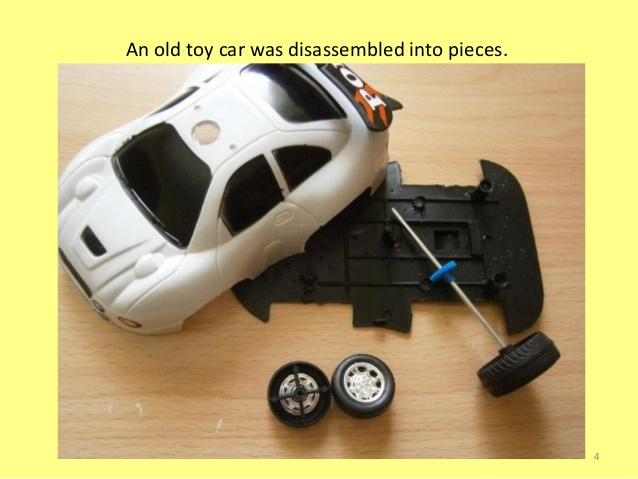
\includegraphics[width=0.7\textwidth]{img/disassembled-toy-car}
  \end{figure}
  \begin{center}
    \tiny
    \url{https://www.slideshare.net/cristinakesh/solar-powered-car-e}
  \end{center}
\end{frame}

\begin{frame}{Me as a Breaker, Repairman, Improver}
  \begin{itemize}
    \pause \item pretty scared as a child
    \pause \item didn't break things on purpose
    \pause \item but it happens
  \end{itemize}
\end{frame}

\begin{frame}{Wired Toy Car Hack}
  % wired toy car
  % bigger battery, instead of 1.5V we used 4.5V
  \begin{figure}
    \centering
    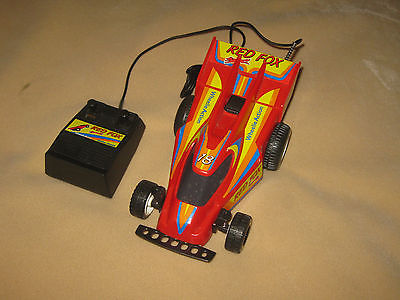
\includegraphics[width=0.7\textwidth]{img/wired-toy-car}
  \end{figure}
  \begin{center}
    \tiny
    \url{https://bricks.stackexchange.com/questions/6755/how-do-i-make-a-remote-control-car-without-lego-motors}
  \end{center}
\end{frame}

\begin{frame}{Rambo Joystick Continuous Repairing}
  % Rambo joystick
  % heat screwdriver, use glue, stick it together
  \begin{figure}
    \centering
    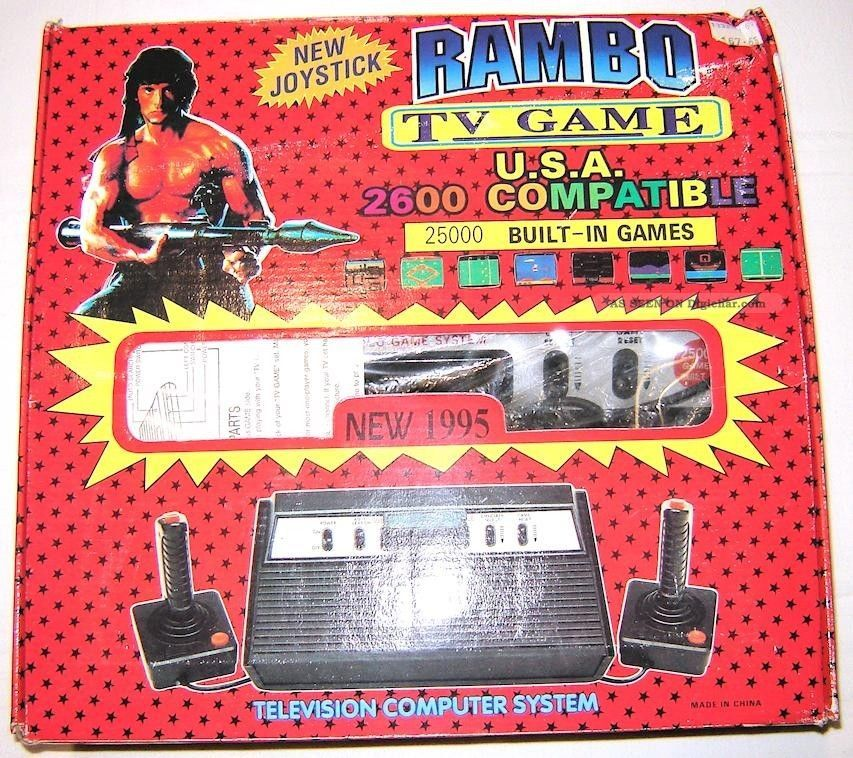
\includegraphics[width=0.6\textwidth]{img/rambo-joystick}
  \end{figure}
  \begin{center}
    \tiny
    \url{https://www.digitiser2000.com/main-page/top-10-funny-console-knock-offs}
  \end{center}
\end{frame}

\begin{frame}{Diablo-affected Mouse Button}
  % Diablo-used mouse
  % middle mouse button, no wheel
  \begin{figure}
    \centering
    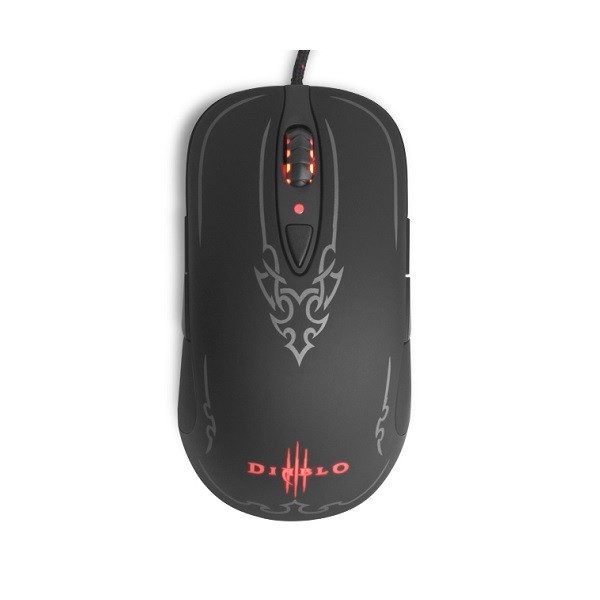
\includegraphics[width=0.5\textwidth]{img/diablo-mouse}
  \end{figure}
  \begin{center}
    \tiny
    \url{https://www.i-tech.com.au/steelseries-diablo-iii-reaper-of-souls-5700dpi-gaming-mouse-ss-62151.html}
  \end{center}
\end{frame}

\begin{frame}{Disembodied PC}
  % disassemble PC
  % all parts on the floor
  % put it all back, it worked the first time
  \begin{figure}
    \centering
    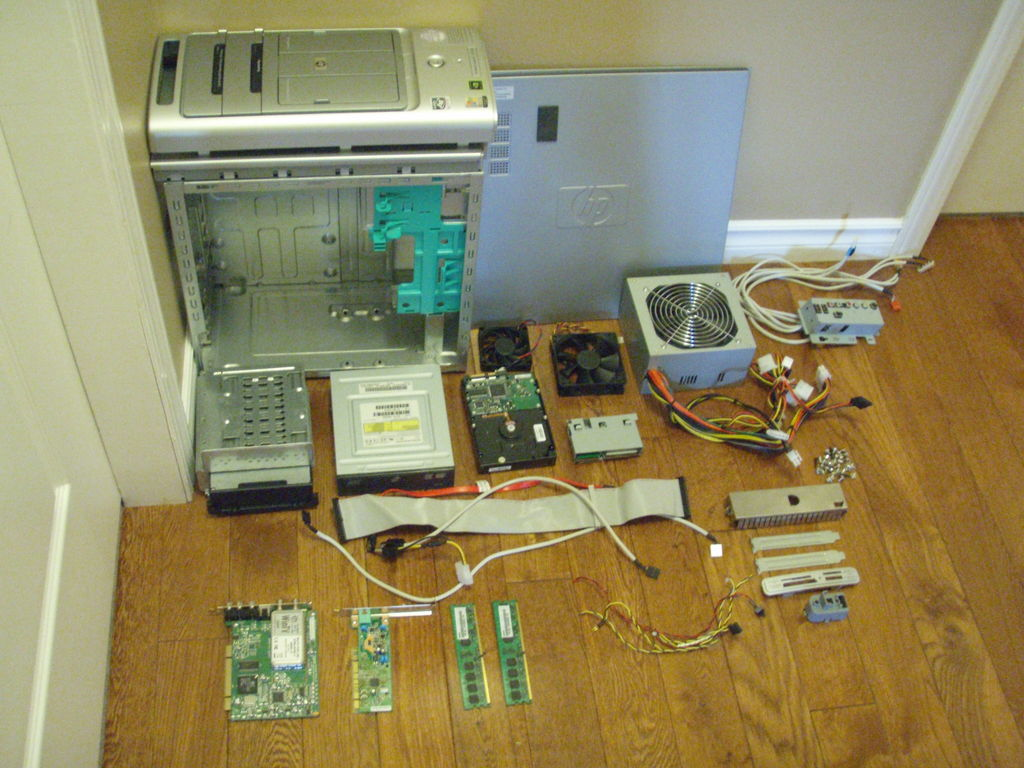
\includegraphics[width=0.7\textwidth]{img/disassembled-pc}
  \end{figure}
  \begin{center}
    \tiny
    \url{https://www.instructables.com/id/Disassemble-a-Computer/}
  \end{center}
\end{frame}

\begin{frame}{Why?}
  \centering
  \pause \Large{Why do kids break stuff?} \\
  \vspace{0.5cm}
  \pause \Large{Why do people break stuff?}
  \vspace{0.5cm}
\end{frame}

\begin{frame}{Why? (2)}
  \centering
  \pause \Large{innate curiosity} \\
  \vspace{0.5cm}
  \pause \Large{desire to look inside, to know how it works} \\
  \vspace{0.5cm}
  \pause \Large{feels good when we know} \\
  \vspace{0.5cm}
  \pause \Large{feels better when we repair} \\
  \vspace{0.5cm}
  \pause \Large{achievement, accomplishment, improvement} \\
  \vspace{0.5cm}
  \pause \Large{goal, purpose}
\end{frame}

\begin{frame}{Dan Pink: Drive}
  \begin{figure}
    \centering
    
\includegraphics[width=0.3\textwidth]{img/drive}
  \end{figure}
  \begin{center}
    \tiny
    \url{https://www.amazon.co.uk/Drive-Daniel-H-Pink/dp/184767769X}
  \end{center}
  \vspace{0.5cm}
  \centering
  \pause autonomy, mastery, purpose
\end{frame}

\begin{frame}{Linus Torvalds and Linux}
  \begin{figure}
    \centering
    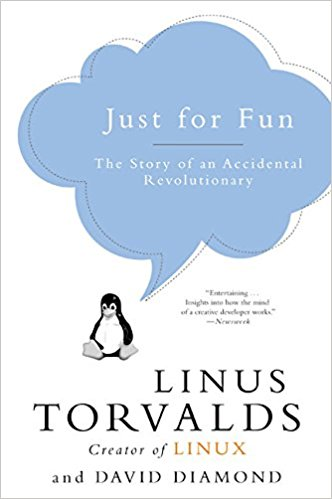
\includegraphics[width=0.3\textwidth]{img/just-for-fun}
  \end{figure}
  \begin{center}
    \tiny
    \url{https://www.amazon.co.uk/Just-Fun-Story-Accidental-Revolutionary/dp/0066620732}
  \end{center}
\end{frame}

\begin{frame}{Really?}
  \centering
  \pause \url{https://www.howstuffworks.com} \\
  \vspace{0.5cm}
  \pause podcasts, YouTube channel \\
  \vspace{0.5cm}
  \pause \url{https://reverseengineering.stackexchange.com}
\end{frame}

\begin{frame}{What is Reversing / Reverse Engineering?}
  \begin{figure}
    \centering
    
\includegraphics[width=0.7\textwidth]{img/reverse-engineering}
  \end{figure}
  \begin{center}
    \tiny
    \url{https://www.wisewhysofsales.com/2017/01/10/reverse-engineering-a-sale/}
  \end{center}
\end{frame}

\begin{frame}{Reversing Targets}
  \centering
  \pause \Large{programs} \\
  \vspace{0.5cm}
  \pause \Large{data formats} \\
  \vspace{0.5cm}
  \pause \Large{protocols}
\end{frame}

\begin{frame}{Andrew Tridgell and Samba}
  \begin{figure}
    \centering
    
\includegraphics[width=0.7\textwidth]{img/samba}
  \end{figure}
  \begin{center}
    \tiny
    \url{https://commons.wikimedia.org/wiki/File:Logo_Samba_Software.svg}
  \end{center}
\end{frame}

\begin{frame}{Why Break Programs?}
  \centering
  \begin{figure}
    \centering
    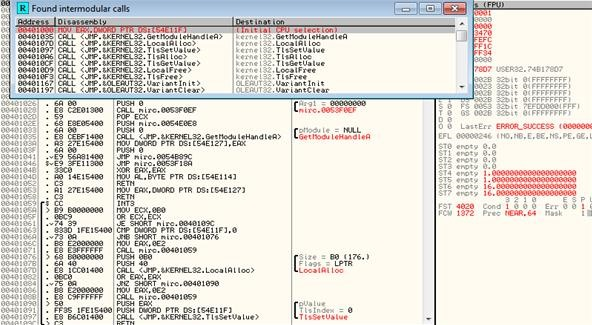
\includegraphics[width=0.7\textwidth]{img/software-cracking}
  \end{figure}
  \begin{center}
    \tiny
    \url{https://null-byte.wonderhowto.com/how-to/hacks-behind-cracking-part-1-bypass-software-registration-0132568/}
  \end{center}
  \pause know how they work \\
  \pause for fun \\
  \pause for fame and glory \\
  \pause hackers, crackers, white/black hat, ethical
\end{frame}

\begin{frame}{Public Hacking/Cracking}
  \centering
  \pause \url{https://www.blackhat.com} \\
  \vspace{0.5cm}
  \pause \url{https://www.defcon.org} \\
  \vspace{0.5cm}
  \pause \url{http://www.hitb.org} \\
\end{frame}

\begin{frame}{Is It Easy?}
\end{frame}

\begin{frame}{Is It Easy?}
  \begin{figure}
    \centering
    
\includegraphics[width=0.7\textwidth]{img/no}
  \end{figure}
  \begin{center}
    \tiny
    \url{https://imgur.com/gallery/DKUR9Tk}
  \end{center}
\end{frame}

\begin{frame}{Is It Easy?}
  \begin{figure}
    \centering
    
\includegraphics[width=0.7\textwidth]{img/hell-no}
  \end{figure}
  \begin{center}
    \tiny
    \url{https://me.me/i/meme-facebook-funny-memes-54435}
  \end{center}
\end{frame}

\begin{frame}{Is It Easy?}
  \begin{figure}
    \centering
    
\includegraphics[width=0.7\textwidth]{img/hell-the-f-no}
  \end{figure}
  \begin{center}
    \tiny
    \url{http://www.ozpolitic.com/cgi-bin/album.pl?photo=forum-attachments/-hell-the-f-no.jpg}
  \end{center}
\end{frame}

\begin{frame}{}
  \pause \textit{Reverse engineering can be depressing and quite solitary. The support from all of you @vu5ec was always there :-), I appreciate the encouragement that I got throughout the process. It was painfully fun!} \\
  \hfill Lucian Cojocar \\
  \vspace{0.5cm}
  \pause \textit{Reversing is like catching a cobra by the back legs.} \\
  \hfill Răzvan Deaconescu
\end{frame}

\begin{frame}{My Story}
  \begin{figure}
    \centering
    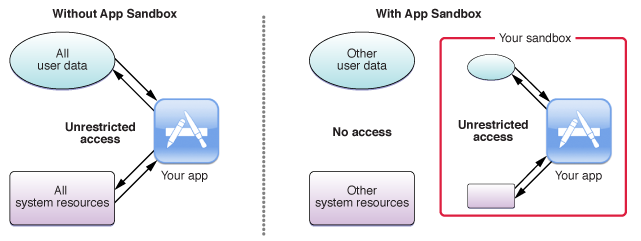
\includegraphics[width=0.8\textwidth]{img/ios-sandboxing}
  \end{figure}
  \begin{center}
    \tiny
    \url{https://developer.apple.com/library/archive/documentation/Security/Conceptual/AppSandboxDesignGuide/AboutAppSandbox/AboutAppSandbox.html}
  \end{center}
\end{frame}

\begin{frame}{Sandboxing}
  \begin{itemize}
    \pause \item limit actions for processes / applications; i.e. open a file, connect to a remote host
    \pause \item in iOS, there are sandbox profiles attached to applications
    \pause \item a sandbox profile contains a specific set of rules
    \pause \item \texttt{container} sandbox profile used for \textbf{all} 3rd party apps (i.e. those installed from Apple AppStore)
  \end{itemize}
\end{frame}

\begin{frame}[fragile]{Initial Format of iOS Sandbox Profiles}
  \begin{alltt}
(version 1)
(allow default)
(deny network*
        (local ip "*:*"))
(deny network-outbound
        (literal "/private/var/tmp/launchd/sock")
        (regex #"^/private/tmp/launchd-[0-9]+[.][^/]+/"))
  \end{alltt}
\end{frame}

\begin{frame}[fragile]{Deployed Format of iOS Sandbox Profiles}
  \begin{alltt}
00000000: 0080 5c9c 9f00 849c 0300 8c00 859c 0000
00000010: 5b9c 5b9c 5b9c 5b9c 5b9c 5b9c 5b9c 5b9c
00000020: 5b9c 5b9c 579c fe9b 5a9c f39b 5b9c 5b9c
00000030: 5b9c 959b 939b 6b9b 959b 5b9c 5b9c 5b9c
00000040: 4f9b 4f9b 4f9b 459b 4f9b 439b 4f9b 4f9b
00000050: 4f9b 4f9b 359b 5b9c 5b9c 5b9c 5b9c 5b9c
00000060: 5b9c 5b9c 5b9c 5b9c 349b 5b9c 5a9c 5b9c
00000070: 5b9c 5b9c 5b9c 5b9c 339b 5b9c 5b9c 5b9c
00000080: 329b 309b 309b 309b 329b 329b 2f9b 2f9b
00000090: 5b9c 5b9c 5b9c 5b9c 5b9c 5b9c 5b9c 5b9c
[...]
  \end{alltt}
\end{frame}

\begin{frame}{Reversing the iOS Sandbox}
  \begin{figure}
    \centering
    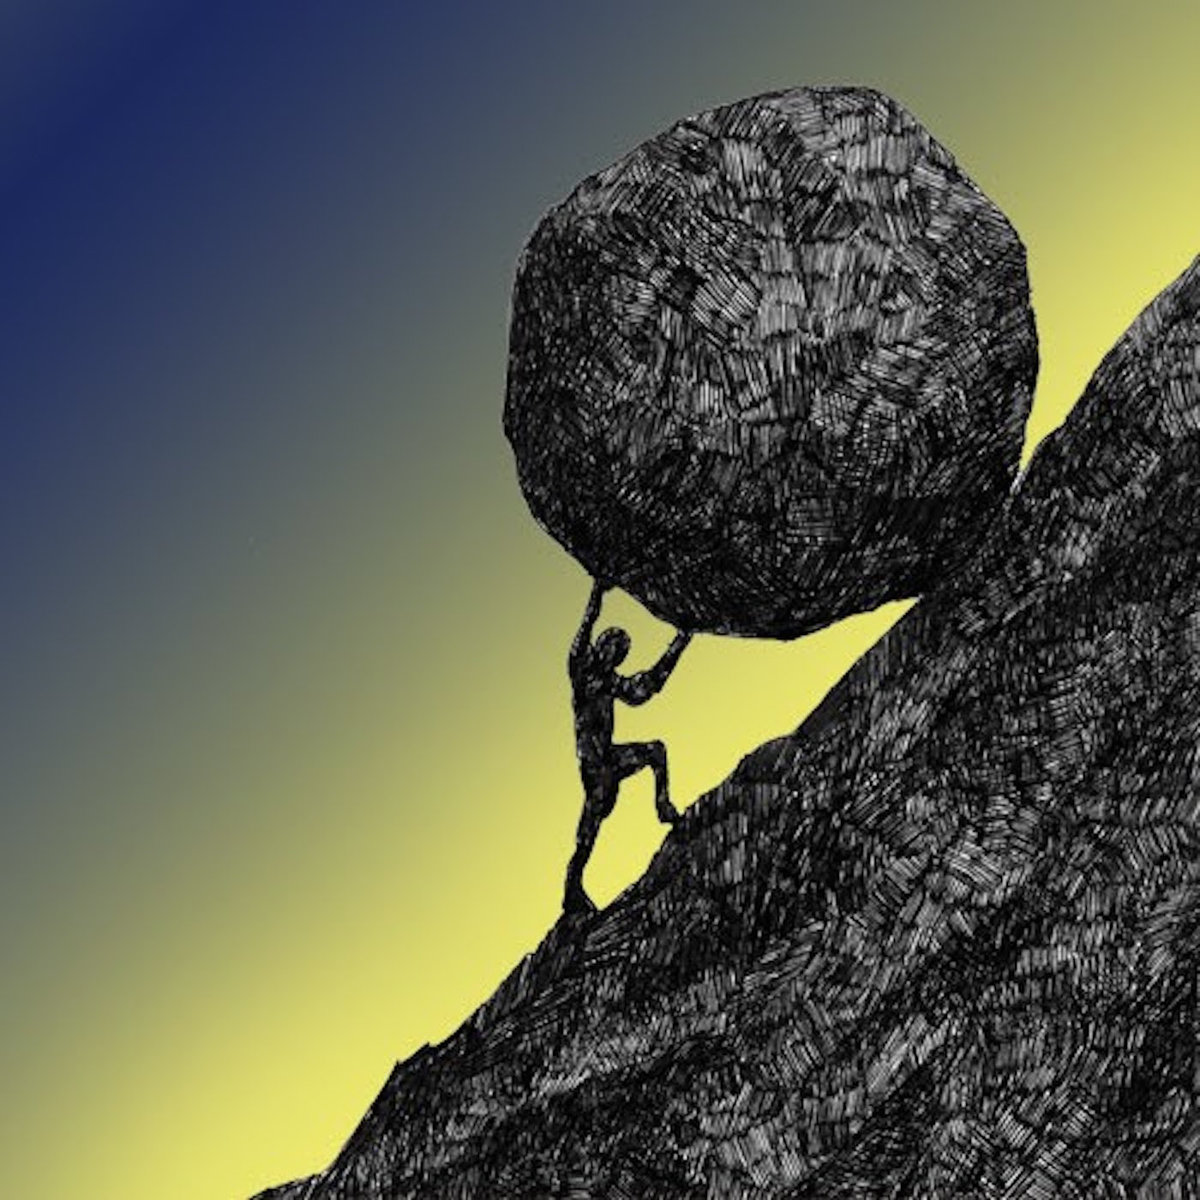
\includegraphics[width=0.5\textwidth]{img/sisyphus}
  \end{figure}
  \begin{center}
    \tiny
    \url{https://coryseznec.bandcamp.com/track/sisyphus}
  \end{center}
  \vspace{0.5cm}
  \pause SandBlaster
  \begin{itemize}
    \item \pause \url{https://arxiv.org/abs/1608.04303}
    \item \pause \url{https://github.com/malus-security/sandblaster}
  \end{itemize}
\end{frame}

\begin{frame}{The Journey}
  \begin{itemize}
    \pause \item close to an year to get it working
    \pause \item another half year to make it work on almost all cases
    \pause \item relentless back-and-forth
    \pause \item made it open source
    \pause \item relied on previous work (Dionysus Blazakis, Stefan Esser, Dino Dai Zovi)
  \end{itemize}
\end{frame}

\begin{frame}{Some other things}
  \begin{itemize}
    \pause \item CTF security contests (Capture the Flag)
    \pause \item master classes on security (open content)
      \begin{itemize}
        \pause \item \url{https://ocw.cs.pub.ro/courses/cns}
        \pause \item \url{http://elf.cs.pub.ro/sis/}
      \end{itemize}
    \pause \item security summer school (open content): \url{https://security.cs.pub.ro/summer-school/wiki/}
  \end{itemize}
\end{frame}

\begin{frame}{Yes but \ldots}
  \centering
  \pause \ldots{} it seems daunting \\
  \pause \ldots{} it takes time
\end{frame}

\begin{frame}{However \ldots}
  \centering
  \pause it will be fun \\
  \pause you will improve: patience, perseverence, lateral thinking, problem solving \\
  \pause you are part of a community
\end{frame}

\begin{frame}{What To Do?}
  \begin{itemize}
    \item \pause CTF contents
      \begin{itemize}
        \item \pause \url{https://picoctf.com}
        \item \pause \url{https://junior.35c3ctf.ccc.ac/announcements/}
        \item \pause \url{https://ctftime.org}
        \item \pause \url{http://captf.com/practice-ctf/}
      \end{itemize}
    \item \pause wargames
      \begin{itemize}
        \item \pause \url{http://io.netgarage.org}
        \item \pause \url{http://smashthestack.org/wargames.html}
        \item \pause \url{http://overthewire.org/wargames/}
      \end{itemize}
  \end{itemize}
\end{frame}

\begin{frame}{Professional Reverse Engineers}
  \centering
  \pause fame, glory \\
  \vspace{0.5cm}
  \pause money \\
  \vspace{0.5cm}
  \pause training \\
  \vspace{0.5cm}
  \pause note legal aspects \\
  \vspace{0.5cm}
  \pause responsible disclosure
\end{frame}

\begin{frame}{Yeah, but ...}
  \centering
  \pause I'm more of a developer \\
  \vspace{0.5cm}
  \pause I want to build stuff, not break stuff \\
  \vspace{0.5cm}
  \pause I want to create
\end{frame}

\begin{frame}{Perspective}
  \pause Sergiu Weisz, 1st year master student \\
  \vspace{0.5cm}
  \pause \textit{I want to build. But I choose to do security because it gives me a better understanding of how things work. And how things can be attacked, abused and brought down.} \\
  \vspace{0.5cm}
  \pause poorly built software, hardware and infrastructure \\
  \vspace{0.5cm}
  \pause you can make it better, more secure, more robust \\
  \vspace{0.5cm}
  \pause once you understand it's inner working
\end{frame}

\begin{frame}{}
  \centering
  \LARGE{Build it. \pause Break it. \pause Make it better.}
\end{frame}

\begin{frame}{Resources}
  \begin{itemize}
    \item mine
      \begin{itemize}
        \item slides: \url{https://www.slideshare.net/razvandeaconescu/}
        \item \url{https://ocw.cs.pub.ro/courses/cns}
        \item \url{http://elf.cs.pub.ro/sis/}
        \item \url{https://security.cs.pub.ro/summer-school/wiki/}
        \item \url{https://arxiv.org/abs/1608.04303}
        \item \url{https://github.com/malus-security/sandblaster}
      \end{itemize}
    \item conferences, events, magazines
      \begin{itemize}
        \item \url{https://www.blackhat.com}
        \item \url{https://www.defcon.org}
        \item \url{http://www.hitb.org}
        \item \url{http://phrack.org/}
      \end{itemize}
  \end{itemize}
\end{frame}

\begin{frame}{Resources (2)}
  \begin{itemize}
    \item CTFs, wargames
      \begin{itemize}
        \item \url{https://picoctf.com}
        \item \url{https://junior.35c3ctf.ccc.ac/announcements/}
        \item \url{https://ctftime.org}
        \item \url{http://captf.com/practice-ctf/}
        \item \url{http://io.netgarage.org}
        \item \url{http://smashthestack.org/wargames.html}
        \item \url{http://overthewire.org/wargames/}
      \end{itemize}
    \item misc
      \begin{itemize}
        \item \url{https://www.amazon.co.uk/Drive-Daniel-H-Pink/dp/184767769X}
        \item \url{https://www.amazon.co.uk/Just-Fun-Story-Accidental-Revolutionary/dp/0066620732}
        \item \url{https://reverseengineering.stackexchange.com}
        \item \url{https://www.howstuffworks.com}
      \end{itemize}
  \end{itemize}
\end{frame}

\end{document}
